\seccion{Transformaci\'on de variables y vectores aleatorios}
\label{Sec:MP:Transformacion}

En esta secci\'on nos interesamos en  los efectos sobre una variable o un vector
aleatorio. Por ejemplo, en un juego con dos dados, nos puede interesar la ley de
la suma que dar\'ia el n\'umero de  casilla que debemos adelantar en un juego de
la oca.
%
\begin{teorema}[Transformaci\'on medible de un vector aleatorio]
\label{Teo:MP:TransformacionMedible}
%
  Sea  \  $X:  (\Omega,\A)  \mapsto  (\Rset^d ,  \B(\Rset^d))$  \  una  variable
  aleatoria,   y  \   $g:  (\Rset^d   ,  \B(\Rset^d))   \mapsto   (\Rset^{d'}  ,
  \B(\Rset^{d'}))$ \  una funci\'on  medible. Entonces,  \ $Y =  g(X)$ \  es una
  variable aleatoria  \ $(\Omega,\A)  \mapsto (\Rset^{d'} ,  \B(\Rset^{d'}))$. \
  Adem\'as, la medida imagen \ $P_Y$ \ est\'a vinculada \ a \ $P_X$ \ por
  %
  \[
  \forall \, B \in \B(\Rset^{d'}), \quad P_Y(B) = P_X(g^{-1}(B)).
  \]
\end{teorema}
%
\begin{proof}
  Este  resultado   es  obvio.  Siendo  $g$  una   funci\'on  medible  (recordar
  Def.~\ref{Def:MP:FuncionMedible}),  para  todo  $B  \in  \B(\Rset^{d'})$,  por
  definici\'on $g^{-1}(B) \in \B(\Rset^d)$.  Adem\'as, si $P_X$ es la medida (de
  probabilidad)  asociada  al  espacio  de   salida  de  $g$,  el  resultado  es
  consecuencia del teorema de la medida imagen~\ref{Teo:MP:MedidaImagen}.
  % , pagina~\pageref{Teo:MP:MedidaImagen}.
\end{proof}
%
\noindent (Ver ej.~\cite{Muk00, JacPro03, AthLah06, Bog07:v2, Coh13}).

Es  sencillo probar  que  cualquier combinaci\'on  de  funciones medibles  queda
medible, cualquier  producto (adecuado) de  funciones medibles queda  medible, y
que si  $\{ f_k \}_{k=1}^{d'}$  son $(\B(\Rset^d),\B(\Rset))$-medibles, entonces
$f        =        (f_1        ,        \ldots       ,        f_{d'})$        es
$(\B(\Rset^d),\B(\Rset^{d'}))$-medible~\cite{AthLah06}.

% \SZ{No se  todav\'ia si ser\'a \'util  tratar del caso de l\'imite  de series de
%   funciones medibles.}


Mencionamos   que si  $\X =  X(\Omega)$ es  discreto, entonces  $\Y =  g(\X) =
Y(\Omega)$ ser\'a discreto tambi\'en, y:
%
\begin{teorema}[Funci\'on de masa por transformaci\'on medible]
\label{Teo:MP:TransformacionMasa}
%
  Sean   $X$,   vector  aleatorio   $d$-dimensional   discreto,  $g:(\Rset^d   ,
  \B(\Rset^d)) \mapsto (\Rset^{d'} , \B(\Rset^{d'}))$ una funci\'on medible, e \
  $Y =  g(X)$ necesariamente discreto  $d'$-dimensional sobre $\Y =  g(\X)$.  La
  distribuci\'on de $Y$ est\'a vinculada con la de $X$ por la relaci\'on
  %
  \[
  \forall \, y \in \Y, \quad p_Y(y) = \sum_{x \in g^{-1}(y)} p_X(x).
  \]
\end{teorema}
%
\begin{proof}
  El resultado es inmediato.
\end{proof}
%
\noindent En particular,  si $g$ es inyectiva (necesariamente  biyectiva de $\X$
en $\Y$),  el vector  de probabilidad queda  invariante, $p_Y =  p_X$; solamente
cambian los estados.

Es  importante  mencionar que  con  $\Y$  discreto,  $\X$ no  es  necesariamente
discreto~\cite{AthLah06}. Por ejemplo, $Y = \un_{X>0}$  es tal que $\Y = \{ 0 \;
1 \}$ a pesar de que $\X$ puede no ser discreto.

Tratar con  variables aleatorias continuas  resulta m\'as delicado. Vimos  en el
ejemplo   precedente   que   el   car\'acter   continuo   puede   perderse   por
transformaci\'on. De  la misma manera, en  un ejemplo de  la secci\'on anterior,
vimos  que  $Y =  X_1  \un_{X_2>0}$ con  $X_i$  independientes  uniformes no  es
continua  ni  discreta.   En  el  enfoque  de  variables  continuas,  una  clase
importante de  funciones en las cuales  nos vamos a interesar  son las funciones
continuas (y diferenciables):
%
\begin{lema}[Continuidad y car\'acter medible]
\label{Lem:MP:ContinuidadCaracterMedible}
%
  Sea   $g:   \Rset^d   \mapsto   \Rset^{d'}$   continua.   Entonces,   $g$   es
  $(\B(\Rset^d),\B(\Rset^{d'}))$-medible.
\end{lema}
%
\begin{proof}
  Por continuidad,  la pre-imagen de  un abierto de  $\Rset^{d'}$ por $g$  es un
  abierto  de $\Rset^d$  y entonces  es en  $\B(\Rset^d)$. La  prueba  se cierra
  recordando  la definici\'on  de $\B(\Rset^{d'})$,  $\sigma$-\'algebra generada
  por los abiertos de $\Rset^{d'}$.
\end{proof}

En lo que sigue, nos interesamos m\'as especialmente en el caso de funciones $g:
(\Rset^d ,  \B(\Rset^d)) \mapsto (\Rset^d ,  \B(\Rset^d))$.  De hecho,  si $d' <
d$,   es    sencillo   llegar    al   caso   considerado    a\~nadiendo   $d-d'$
transformaciones. Por ejemplo, con $d = 2$ si nos interesa $X_1 + X_2$, se puede
considerar $\begin{bmatrix} X_1 + X_2 &  X_2 - X_1\end{bmatrix}^t$ y llegar a la
variable de inter\'es  por c\'alculo de marginal. Si $d' >  d$ la situaci\'on es
m\'as  delicada,   $g(Y)$  viviendo   sobre  una  variedad   $d$-dimensional  de
$\Rset^{d'}$.

En el  caso de vectores  aleatorios continuos $X$  que admitend una  densidad de
probabilidad,  una  pregunta  natural  es  entonces  saber  si  se  conserva  la
continuidad y la  existencia de una densidad, as\'i como  su forma. La respuesta
se da en el teorema siguiente~\cite{Bre88, JacPro03, AthLah06, Coh13, HogMck13}:
%
\begin{teorema}[Densidad de probabilidad por transformaci\'on continua inyectiva
  diferenciable]\label{Teo:MP:TransformacionInyectivaDensidad}
%
  Sea $X$, vector aleatorio $d$-dimensional  continuo que admite una densidad de
  probabilidad $p_X$, y sea \ $g:\Rset^d \mapsto \Rset^d$ una funci\'on continua
  inyectiva y diferenciable tal que
  %  ~\footnote{\modif{De  hecho,  se   puede  extender  el  resultado  para  un
  %      determinente del  Jacobiano cancelandose  en  un conjunto  de punto  de
  %     medida  de Lebesgue nula y en  los $y$ donde se  cancela el determinente
  %       del  Jacobiano,  la   densidad  va   a  ser   divergente  (divergencia
  %     integrable).}}
  $\left| \Jac_g \right| > 0$ (ver notaciones),
  %
  % donde   $\Jac_g$  denota   la  matriz   de  componentes   \  $\frac{\partial
  %   g_i}{\partial  x_j}$,  \ matriz  Jacobiana  de  la  transformaci\'on \  $g
  % \equiv \begin{bmatrix} g_1(x_1 , \ldots , x_d) & \cdots & g_d(x_1 , \ldots ,
  %   x_d) \end{bmatrix}^t$  \ y  \ $|\cdot|$ representa  el valor  absoluto del
  % determinante de la matriz.
  Sea  \  $Y =  g(X)$.   Entonces  $Y$ es  continua  y  admite  una densidad  de
  probabilidad $p_Y$ de soporte $\Y = g(\X) = Y(\Omega)$ tal que
  %
  \[
  \forall \,  y \in  \Y, \quad p_Y(y)  = p_X(g^{-1}(y))  \left| \Jac_{g^{-1}}(y)
  \right|.
  \]
\end{teorema}
%
\begin{proof}
  Por definici\'on, admitiendo $X$ una densidad y  siendo $g$ medible,
  %
  \[
  \forall \, B \in \B(\Rset^d),  \quad P_Y(B) = P_X(g^{-1}(B)) = \int_{g^{-1}(B)
    \cap \X} p_X(x) \, dx.
  \]
  %
  Por cambio de variables $x  = g^{-1}(y)$ (siendo $g$ inyectiva, el antecedente
  es \'unico por definici\'on) y  notando que $g\left( g^{-1}(B) \cap \X \right)
  = B \cap \Y$,
  %
  \[
  \forall \, B  \in \B(\Rset^d), \quad P_Y(B) =  \int_{B \cap \Y} p_X(g^{-1}(y))
  \, \left| \Jac_{g^{-1}}(y) \right| \, dy
  \]
  %
  lo que cierra la prueba~\footnote{La aparici\'on del Jacobiano viene del mismo
    enfoque que el cambio de variables en la integraci\'on de Riemann. De hecho,
    como lo  hemos visto, $\mu_L(B)  = |B|$ es  el volumen y de  la definici\'on
    misma del determinente, para cualquier matriz cuadrada el volumen se escribe
    \ $\mu_L(M  B) = |M B|  = |M| |B| =  |M| \mu_L(B)$ donde  la misma escritura
    $|\cdot|$ representa el valor absoluto  del determinente de una matriz. Esta
    notaci\'on se justifica precisamente por su significaci\'on de volumen, y el
    resultado   es  inmediato  para   $g(x)  =   M  x$.    La  forma   para  una
    transformaci\'on m\'as general se obtiene a partir de un desarollo de Taylor
    al orden  1 de  la transformaci\'on, haciendo  aparecer el  determinente del
    Jacobiano~\cite{AthLah06, Coh13}.}.
\end{proof}

El caso escalar puede ser visto como caso particular, dando:
%
\begin{corolario}
\label{Cor:MP:TransformacionInyectivaDensidadEscalar}
%
  Sean $X$, variable aleatoria continua  que admite una densidad de probabilidad
  $p_X$,   $g:\Rset  \mapsto   \Rset$  una   funci\'on  continua,   inyectiva  y
  diferenciable, e \ $Y = g(X)$.  Entonces $Y$ es continua y admite una densidad
  de probabilidad $p_Y$ tal que
  %
  \[
  \forall  \,   y  \in  \Y,   \quad  p_Y(y)  =  p_X(g^{-1}(y))   \left|  \frac{d
      g^{-1}(y)}{dy} \right|.
  \]
\end{corolario}
%
\noindent De hecho,  se pueden ver estos resultados  esquem\'aticamente como una
``conservaci\'on'' de  probabilidad, $p_X(x)  dx = p_Y(y)  dy$, el  volumen $dy$
estando  relacionado al  $dx$  a traves  de  la matriz  Jacobiana  (ver nota  de
pie~\ref{Foot:SZ:Jacobiana}).

Una  forma  alternativa  de derivar  este  corolario  consiste  en salir  de  la
funci\'on    de    repartici\'on,   notando    que    $g$   es    necesariamente
mon\'otona~\footnote{Notar que $P(X \ge x) = 1 - P(X < x) = 1 - P(X \le x) + P(X
  =  x)$, pero  siendo $X$  continua, $  P(X =  x) =  0$.}: si  $y  \notin \Y$,
necesariamente $p_Y = 0$ ($F_Y(y) = 1$ \ si \ $y > \sup \Y$ \ y \ $F_Y(y) = 0$ \
si \ $y < \inf \Y$) \ y para cualquier \ $y \in \Y$,
%
\[
F_Y(y) = P(Y \le y) = P(g(X) \le y) =
\left\{\begin{array}{lll}
P(X \le g^{-1}(y)) = F_X(g^{-1}(y)) & \mbox{si} & g \quad \mbox{es creciente}\\[2.5mm]
%
P(X \ge g^{-1}(y)) = 1 - F_X(g^{-1}(y)) & \mbox{si} & g \quad \mbox{es decreciente}
\end{array}\right..
\]
%
El  resultado  se  obtiene  calculando  las  derivadas  del  primer  y  \'ultimo
t\'erminos respecto de la variable transformada $y$.

Si $g$ no es inyectiva, $g^{-1}$  es multivaluada o multiforme. En este caso, se
puede todav\'ia  tratar el problema, particionando $\Rset^d$  en conjuntos donde
$g$ es inyectiva, dando
%
\begin{teorema}[Densidad   de   probabilidad   por   transformaci\'on   continua
  no inyectiva diferenciable]\label{Teo:MP:TransformacionNoInyectivaDensidad}
%
  Sea $X$, vector aleatorio $d$-dimensional  continuo que admite una densidad de
  probabilidad  $p_X$,  y sea  $g:(\Rset^d  ,  \B(\Rset^d))  \mapsto (\Rset^d  ,
  \B(\Rset^d))$  una  funci\'on continua  y  diferenciable.  Denotamos  $\left\{
    \X_{[k]} \right\}_{k=0}^m$ la partici\'on  de $\X$ tal que $\left| \Jac_g(y)
  \right| = 0$ sobre  $\X_{[0]}$, y para todo $k \ge 1$  se tiene \ $g: \X_{[k]}
  \mapsto  \Y$ \  inyectiva  y tal  que \  $\left|  \Jac_g(y) \right|  > 0$.   \
  Suponemos que $\X_{[0]}$ es de medida \modif{$P_X$} nula, notamos \ $g_k^{-1}$
  \ la funci\'on inversa de \ $g$ \ sobre \ $g(\X_{[k]})$ \ (rama $k$-\'esima de
  la  funci\'on   multivaluada  $g^{-1}$),  \  $\Jac_{g_k^{-1}}$   \  su  matriz
  Jacobiana, e \  $I(y) = \{ k \tq  y \in g(\X_{[k]}) \}$ \  los \'indices tales
  que  \  $y$  \  tiene  un   inverso  por  $g_k$.   Esto  es  ilustrado  en  la
  figura~\ref{Fig:MP:TransformacionVA} para $d = 1$.  Entonces $Y$ es continua y
  admite una densidad de probabilidad $p_Y$ tal que
  %
  \[
  \forall  \, y  \in \Y,  \quad p_Y(y)  = \sum_{k  \in  I(y)} p_X(g_k^{-1}(y))
  \left| \Jac_{g_k^{-1}}(y) \right|.
  \]
  %
  En el caso escalar $d = 1$ esto se formula
  %
  \[
  \forall \, y \in \Y, \quad  p_Y(y) = \sum_{k \in I(y)} p_X(g_k^{-1}(y)) \left|
    \frac{d g_k^{-1}(y)}{dy} \right|.
  \]
  %
  \noindent Esto se ilustra el la figura~\ref{Fig:MP:TransformacionVA}.
\end{teorema}
%
\begin{proof}
  \modif{Basta escribir \  $g^{-1}(B) = \bigcup_{k = 0}^m  \left( g^{-1}(B) \cap
      \X_{[k]} \right)$, uni\'on de borelianos disjuntos. Siendo $g^{-1}(B) \cap
    \X_{[k]} = g_k^{-1}(B)$, y siendo $\X_{[0]}$ de medida nula, se obtiene
  %
  \[
  P_Y(B) = P_X(g^{-1}(B)) = \sum_{k=1}^m \int_{g_k^{-1}(B)} p_X(x) \, dx
  \]
  %
  Se  nota ahora  que $g_k(g_k^{-1}(B)) = B \cap g(\X_{[k]})  \subset  B$ pero  no es  necesariamente
  $B$. Sin embargo, Por cambio de variables $x = g_k^{-1}(y)$ en cada integral, tenemos intonces
  %
  \[
  P_Y(B)  =   \sum_{k=1}^m \int_{B \cap g(\X_{[k]})}
  p_X\left( g_k^{-1}(y) \right) \left| \Jac_{g_k^{-1}}(y) \right| \, dy  =   \int_B
  \sum_{k=1}^m  \un_{g(\X_{[k]})}(y) \, p_X\left( g_k^{-1}(y) \right) \left| \Jac_{g_k^{-1}}(y) \right| \, dy
  \]
  %
  Por definici\'on de $I(y)$, $y \in B \cap g(\X_{[k]}) \:\: \Leftrightarrow \:\: k \in I(y) $, lo conduce finalmente a
  %
  \[
  P_Y(B)  = \int_{B \cap  g(\X_{[k]})} \sum_{k  \in I(y)}  p_X\left( g_k^{-1}(y)
  \right) \left| \Jac_{g_k^{-1}}(y) \right| \, dy
  \]
 }
 % Basta escribir \ $B = \bigcup_{k  = 0}^m \left( B \cap g(\X_{[k]}) \right)$ \
 % uni\'on de  borelianos disjuntos, notar  que por consecuencia \  $g^{-1}(B) =
 % \bigcup_{k  =0}^m  g^{-1}\left( B  \cap  g(\X_{[k]})  \right)$  \ uni\'on  de
 % borelianos disjuntos  \ y  \ por linealidad  escribir la  integraci\'on sobre
 % $g^{-1}(B)$ como la suma de integrales sobre $g^{-1}\left( B \cap g(\X_{[k]})
 % \right)$. Se cierra la prueba  notando que \ $g^{-1}\left( B \cap g(\X_{[0]})
 % \right)$ es  necesariamente de  medida de Lebesgue  nula, siendo  la integral
 % nula y que \ $g^{-1}\left( B \cap g(\X_{[k]}) \right) = g_k^{-1}\left( B \cap
 %   g(\X_{[k]}) \right)$.
\end{proof}

\begin{figure}[h!]
\begin{center} 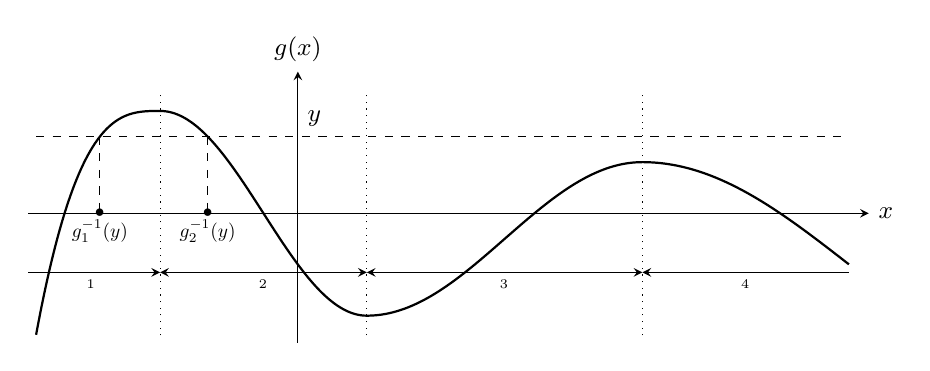
\begin{tikzpicture}%[scale=.9]
\shorthandoff{>}
%
\pgfmathsetmacro{\sx}{1.75};% x-scaling
%
% transformacion g' = 0 medida nula
\begin{scope}
%
\pgfmathsetmacro{\sy}{1.3};% y-scaling 
%
\draw[>=stealth,->] ({-1.9*\sx-.1},0)--({\sx*4+.25},0) node[right]{\small $x$};
\draw[>=stealth,->] (0,{\sy*(-3*.9^3+1)-.1})--(0,{\sy+.5}) node[above]{\small $g(x)$};
%
\draw[thick]
plot[domain=-1.9:-1,samples=100] ({\sx*\x},{\sy*(3*(\x+1)^3+1)})
-- plot[domain=-1:.5,samples=100] ({\sx*\x},{\sy*cos(120*(\x+1))})
-- plot[domain=.5:2.5,samples=100] ({\sx*\x},{\sy*(.75*sin(90*(\x-1.5))-.25)})
-- plot[domain=2.5:4,samples=100] ({\sx*\x},{\sy*(cos(60*(\x-2.5))-.5)})
;
%
\draw[dashed] ({-1.9*\sx},{.75*\sy})--({4*\sx},{.75*\sy});
\draw (0,{.75*\sy}) node[above right]{\small $y$};
%
\draw[dashed] ({-\sx*(1+(.25/3)^(1/3))},{.75*\sy})--({-\sx*(1+(.25/3)^(1/3))},0)
node[scale=.7]{$\bullet$} node[below,scale=.7]{$g_1^{-1}(y)$};
%
\draw[dashed] ({\sx*(acos(.75)/120-1)},{.75*\sy})--({\sx*(acos(.75)/120-1)},0)
node[scale=.7]{$\bullet$} node[below,scale=.7]{$g_2^{-1}(y)$};
%
%
\draw[dotted] ({-\sx},{-\sy-.25})--({-\sx},{\sy+.25});
\draw[>=stealth,->] ({-\sx*1.9-.1},-.75)--({-\sx},-.75);
\draw ({-1.5*\sx},-.75) node[below,scale=.8]{\small $\X_1$};
%
\draw[dotted] ({.5*\sx},{-\sy-.25})--({.5*\sx},{\sy+.25});
\draw[>=stealth,<->] ({-\sx},-.75)--({.5*\sx},-.75);
\draw ({-.25*\sx},-.75) node[below,scale=.8]{\small $\X_2$};
%
\draw[dotted] ({2.5*\sx},{-\sy-.25})--({2.5*\sx},{\sy+.25});
\draw[>=stealth,<->] ({.5*\sx},-.75)--({2.5*\sx},-.75);
\draw ({1.5*\sx},-.75) node[below,scale=.8]{\small $\X_3$};
%
\draw[>=stealth,<-] ({2.5*\sx},-.75)--({4*\sx},-.75);
\draw ({3.25*\sx},-.75) node[below,scale=.8]{\small $\X_4$};
\end{scope}
%
%
% % reparticion
% \begin{scope}[xshift=8.5cm]
% %
% \pgfmathsetmacro{\sy}{2};% y-scaling 
% %
% \draw[>=stealth,->] (-.6,0)--({\sx*4+.25},0) node[right]{\small $x$};
% \draw[>=stealth,->] (0,-.25)--(0,{\sy+.5}) node[above]{\small $F_X$};
% %
% \draw[thick] (-.5,0)--(0,0)--(\sx,{\sy/2})--({2*\sx},{\sy/2})
% -- plot[domain=2:3,samples=100] ({\sx*\x},{\sy*(1+(\x-2)^(3/2))/2})
% -- ({\sx*4},\sy);
% %
% \draw (\sx,0)--(\sx,-.1) node[below,scale=.9]{\small $1$};
% \draw ({2*\sx},0)--({2*\sx},-.1) node[below,scale=.9]{\small $2$};
% \draw ({3*\sx},0)--({3*\sx},-.1) node[below,scale=.9]{\small $3$};
% \draw (\sx,0)--(\sx,-.1) node[below,scale=.9]{\small $1$};
% %
% \draw (0,{\sy/2})--(-.1,{\sy/2}) node[left,scale=.7]{\small $1/2$};
% \draw (0,\sy)--(-.1,\sy) node[left,scale=.7]{\small $1$};
% %
% \draw ({\sx*2.25},-1) node{\small (b)};
% \end{scope}
%
\end{tikzpicture} \end{center}
%
\leyenda{Ilustraci\'on  de  una  transformaci\'on  $g$  no  inyectiva,  tal  que
  $\X_{[0]} = \{ x \tq g'(x) = 0 \}$, representado por los valores de $x$ en las
  lineas  punteadas. Es de  medida de  Lebesgue nula.   Se indican  los dominios
  $\X_{[k]}$.  La l\'inea discontinua da un nivel $y$ y los puntos en el eje $x$
  representan $g_k^{-1}(y), \: k \in I(y)$; en el ejemplo, $I(y) = \{ 1 \; 2 \}$
  \  y,   suponiendo  que  $\X  =   \Rset$,  \  $F_Y(y)   =  F_X(g_1^{-1}(y))  +
  1-F_X(g_2^{-1}(y))$.}
\label{Fig:MP:TransformacionVA}
\end{figure}

\begin{ejemplo}[Ejemplo de transformaci\'on no biyectiva]
\label{Ej:MP:TransformacionNoBiyectiva}
%
Sea $X$ definida sobre \ $\X =  \Rset$ \ y la transformaci\'on de variables \ $Y
= X^2$.  Se  tiene \ $y =  g(x) = x^2$, continua diferenciable  de derivada nula
sobre \ $\X_{[0]} = \{ 0 \}$,  de medida nula, cuyas inversas son \ $g_1^{-1}(y)
= - \sqrt{y}$ \ sobre \ $\X_{[1]}  = \Rset_{0,-}$ \ y \ $g_2^{-1}(y)
=   +  \sqrt{y}$   sobre  \   $\X_{[2]}  =   \Rset_{0,+}$;  luego   \   $p_Y(y)  =
\frac{p_X(\sqrt{y}) + p_X(-\sqrt{y})}{2 \sqrt{y}}$, \ sobre \ $\Y = \Rset_{0,+}$.
\end{ejemplo}

De nuevo, en el caso escalar, se puede salir de la funci\'on de repartici\'on
%
\[
F_Y(y) =  P(Y \le y) = P(  g(X) \le y )  = \sum_{k=1}^m P\left( X  \in \X_{[k]} \cap
  g_k^{-1}(-\infty \; y] \right)
\]
%
(siendo  $\X_{[0]}$  de medida  nula,  sobre  este  dominio la  probabilidad  es
cero). Sea $\Y_{[k]} = g_k(\X_{[k]})$. Ahora, si $y \notin I(y)$,
%
\[
P\left(   X   \in  \X_{[k]}   \cap   g_k^{-1}(-\infty  \;   y]  \right)   =
\left\{\begin{array}{lll}
%
P(X \in \X_{[k]}) & \mbox{si} & y > \sup \Y_{[k]}\\[2.5mm]
%
0 & \mbox{si} & y < \inf \Y_{[k]}
\end{array}\right.
\]
%
dando una derivada nula. Si $y \in I(y)$,
%
\[
P\left(   X   \in  \X_{[k]}   \cap   g_k^{-1}(-\infty  \;   y]  \right)   =
\left\{\begin{array}{lll}
%
F_X(g_k^{-1}(y)) - F_X(\inf \Y_{[k]}) & \mbox{si} & g_k \quad \mbox{es creciente}\\[2.5mm]
%
F_X(\sup \Y_{[k]}) - F_X(g_k^{-1}(y))  & \mbox{si} & g_k \quad \mbox{es decreciente}
\end{array}\right..
\]
%
El resultado sigue diferenciando estas expresiones. Se ilustra esto tambi\'en en
la figura~\ref{Fig:MP:TransformacionVA}.

Una tercera alternativa, a pesar de que sea delicado, es apoyarse en la teor\'ia
de distribuciones  y expresar como \  $\displaystyle p_Y(y) =  \int_\X p_X(x) \,
\delta(y-g(x)) \,  dx$, donde  se usa  la expansi\'on de  la funci\'on  delta en
t\'erminos de sus ceros:  \ $\delta(y-g(x)\,)= \sum_{k \in I(y)} \frac{1}{\left|
    g_k'\left(          g_k^{-1}          (y)          \right)          \right|}
\delta(x-g_k^{-1}(y))$~\cite{ManWol95}.

Es  importante   notar  que  la   condici\'on  $\X_{[0]}$  de  medida   nula  es
importante. Al  contrario, $Y$  no resulta  continua como se  puede ver  en el
ejemplo siguiente.
%
\begin{ejemplo}[Transformaci\'on con \modif{$P_X\left( \X_{[0]} \right) \ne 0$}]
\label{Ej:MP:X0MedidaNoNula}
%
Sea \ $X$ \ uniforme sobre  \ $\X = ( 3 \; 3)$ \ e \ $Y  = g(X)$ \ con \ $g(x) =
\Big(  1 +  \cos\left(  (|x|-1) \frac{\pi}{2} \right) \Big)  \un_{(1 \;  3)}(|x|) +  2
  \un_{[0    \;   1]}(|x|)$.     Esta    funci\'on   se    representa   en    la
  figura~\ref{Fig:MP:TransformacionVANoContinua}-(a).   Claramente, \  $g$  \ es
  continua y diferenciable sobre $\X$, pero con \ $\X_{[0]} = [ -1 \; 1]$ que no
  es  de  medida  nula.   Saliendo  de  $F_Y(y) =  P(g(X)  \le  y)$  se  calcula
  sencillamente  $F_Y(y) =  \frac23 \left(  1 -  \frac1\pi  \arccos(y-1) \right)
  \un_{[0   \;   2)}   +   \un_{[   2  \;   +\infty)}(y)$,   ilustrada   en   la
  figura~\ref{Fig:MP:TransformacionVANoContinua}-(b).   Claramente \ $F_Y$  \ es
  discontinua en \ $y = 2$: \ $Y$ \ no es continua.
  %
  \begin{figure}[h!]
  \begin{center} \begin{tikzpicture}%[scale=.9]
\shorthandoff{>}
%
\pgfmathsetmacro{\r}{.05};% radius arc non continuity F_X y/o p_X
%
% transformacion g' = 0 medida no nula
\begin{scope}
%
\draw[>=stealth,->] (-3.6,0)--(3.75,0) node[right]{\small $x$};
\draw[>=stealth,->] (0,-.25)--(0,2.5) node[above]{\small $g(x)$};
%
\draw[thick]
(-3.4,0)--(-3,0)--
plot[domain=-3:-1,samples=100] (\x,{1+cos(90*(1+\x))})--
(1,2)--
plot[domain=1:3,samples=100] (\x,{1+cos(90*(1-\x))})--
(3.5,0);
%
\draw (-3,0)--(-3,-.1) node[below,scale=.8]{\small $-3$};
\draw (-2,0)--(-2,-.1) node[below,scale=.8]{\small $-2$};
\draw (-1,0)--(-1,-.1) node[below,scale=.8]{\small $-1$};
\draw (1,0)--(1,-.1) node[below,scale=.8]{\small $1$};
\draw (2,0)--(2,-.1) node[below,scale=.8]{\small $2$};
\draw (3,0)--(3,-.1) node[below,scale=.8]{\small $3$};
%
\draw (0,1)--(-.1,1) node[left,scale=.8]{\small $1$};
\draw (-.1,2) node[above left,scale=.8]{\small $2$};
%
\draw[>=stealth,<->] (-3,-.5)--(-1,-.5); \draw (-2,-.5) node[below,scale=.9]{\small $\X_{[1]}$};
\draw[>=stealth,<->] (1,-.5)--(3,-.5); \draw (2,-.5) node[below,scale=.9]{\small $\X_{[2]}$};
\draw[>=stealth,<->] (-1,-.5)--(1,-.5); \draw (0,-.5) node[below,scale=.9]{\small $\X_{[0]}$};
%
\draw(0,-1.5) node{\small (a)};
\end{scope}
%
%
% reparticion
\begin{scope}[xshift=7cm]
%
\pgfmathsetmacro{\sx}{1.5};
\pgfmathsetmacro{\sy}{2};% y-scaling 
%
\draw[>=stealth,->] (-.6,0)--({3*\sx+.5},0) node[right]{\small $y$};
\draw[>=stealth,->] (0,-.25)--(0,{\sy+.25}) node[above]{\small $F_Y$};
%
\draw[thick] (-.5,0)--(0,0)--
plot[domain=0:2,samples=250] ({\sx*\x},{\sy*2*(1-acos(\x-1)/180)/3});
%
\draw ({2*\sx+\r},{2*\sy/3+\r}) arc (90:260:\r);
%--
\draw[dotted] ({2*\sx},{2*\sy/3})--({2*\sx},\sy);
\draw[thick] ({2*\sx},\sy) node[scale=.7]{$\bullet$}--({3*\sx},\sy);
%
\draw ({\sx},0)--({\sx},-.1) node[below,scale=.8]{\small $1$};
\draw ({2*\sx},0)--({2*\sx},-.1) node[below,scale=.8]{\small $2$};
\draw ({3*\sx},0)--({3*\sx},-.1) node[below,scale=.8]{\small $3$};
%
\draw (0,{2*\sy/3})--(-.1,{2*\sy/3}) node[left,scale=.7]{\small $2/3$};
\draw (0,\sy)--(-.1,\sy) node[left,scale=.7]{\small $1$};
%
\draw({1.75*\sx},-1.5) node{\small (b)};
\end{scope}
%
\end{tikzpicture} \end{center}
  %
  \leyenda{(a): Gr\'afica de $g(x) =  \Big( 1 + \cos\left( (|x|-1) \frac{\pi}{2}
    \right) \Big) \un_{(1  \; 3)}(|x|) + 2 \un_{[0  \; 1]}(|x|)$. Suponiendo que
    $\X  = (-3  \; 3)$,  claramente $\X_{[0]}  = [  -1 \;  1]$ no  es  de medida
    nula. (b): Para $X$ uniforme sobre  $\X$, la variable $Y = g(X)$ resulta con
    funci\'on de repartici\'on $F_Y$ no continua.  }
  \label{Fig:MP:TransformacionVANoContinua}
  \end{figure}
\end{ejemplo}

Un ejemplo de  cambio de transformaci\'on puede sevir a  calcular la densidad de
probabilidad de una suma:
%
\begin{ejemplo}[Distribuci\'on de la suma de vectores aleatorios]
\label{Ej:MP:Suma}
%
  Sean \ $X$ \ e \ $Y$ \ dos vectores aleatorios $d$-dimensionales conjuntamente
  continuos, de densidad de probabilidad conjunta $p_{X,Y}$, y sea el vector \[V
  = X +  Y.\] Queremos calcular la densidad de probabilidad  de $V$.  Para esto,
  se puede considerar la transformaci\'on biyectiva
  %
  \[
  g: (x,y) \mapsto (u,v) = (x,x+y).
  \]
  %
  Entonces
  %
  \[
  g^{-1}(u,v) = (u,v-u)
  \]
  %
  y la matriz Jacobiana es
  %
  \[
  J_{g^{-1}} = \begin{bmatrix} I & -I \\ 0 & I \end{bmatrix}
  \]
  %
  \modif{donde  la  identidad  \  $I$  \  y  la matriz  nula  \  $0$  \  son  en
    $\M_{d,d}(\Rset)$  conjuntos de  matrices  $d \times  d$ (ver  notaciones)}.
  Claramente\ $\left| J_{g^{-1}} \right| = 1$ \ as\'i que
  %
  \[
  p_{U,V}(u,v) = p_{X,Y}(u,v-u)
  \]
  %
  como lo podiamos intuir. Adem\'as, por marginalizaci\'on, inmediatamente
  %
  \[
  p_V(v) = \int_{\Rset^d} p_{X,Y}(u,v-u) \, du.
  \]
  %
  Si \ $X$ \ e \ $Y$  \ son independientes, \ $p_{U,V}(u,v) = p_X(u) p_Y(v-u)$ \
  y la f\'ormula integral se escribe
  %
  \[
  p_V(v) = \int_{\Rset^d} p_X(u) p_Y(v-u) \, du = \int_{\Rset^d} p_Y(u) p_X(v-u)
  \, du
  \]
  %
  (por  cambio  de variable  en  la  secunda  expresi\'on).  Esta  f\'ormula  es
  conocida    como     {\it    producto    de     convoluci\'on}    entre    las
  funciones~\footnote{\modif{Un  producto  de  convolution  entre  funciones  se
      define entre cualquieras funciones,  que sean densidades de probabilidad o
      no}.  Una  condici\'on suficiente para que existe  \modif{tal producto} es
    que  las funciones \modif{que  se convoluan}  sean $L^1$\modif{~\cite{Gol61,
        SteWei71, Pin09}  (es el caso  de densidad de probabilidad)}.}   $p_X$ y
  $p_Y$ \modif{y como lo podemos ver, es conmutativo}.
\end{ejemplo}
